\section{Theorie}
\label{sec:theorie}

Das Element Rubidium zählt zur Gruppe der Alkalimetalle und ist für den Versuch des Optischen Pumpens deshalb besonders geeignet.
Denn ähnlich wie das Wasserstoffatom besitzen Alkalimetalle nur ein Valenzelektron.
Die anderen Elektronen sind in vollen Schalen und tragen nicht zu dem optischen Pumpen bei.\\
In diesem Versuch werden zwei Isotope des Rubidiums verwendet.
Das stabile Rubidium $^{85}\text{Rb}$ und der radioaktive Beta-Strahler $^{87}\text{Rb}$ liegen als Gas vor.

\subsection{Feinstruktur}
Die Quantenzahlen der beiden Isotope unterscheiden sich kaum, bis auf den Kernspin I.\\
Der Gesamtbahndrehimpuls J berechnet sich aus dem Drehimpuls L und dem Spin S nach $\vec{J} = \vec{L} + \vec{S}$.
Dabei sind die Quantenzahlen gegeben durch $|L-S|$ bis $|L+S|$ in ganzen Schritten.
Im Fall des Rubidium ergibt sich in jedem Fall $J=\sfrac{1}{2}$.
In \autoref{tab:quanten} sind alle Quantenzahlen im Grundzustand ohne Zeeman-Aufspaltung aufgelistet.

\begin{table}[H]
    \centering
    \begin{tabular}{c c c}
        \toprule
        - & $^{85}\text{Rb}$ & $^{87}\text{Rb}$\\
        \midrule
        L & 0 & 0\\
        S & $\sfrac{1}{2}$ & $\sfrac{1}{2}$\\
        J & $\sfrac{1}{2}$ & $\sfrac{1}{2}$\\
        I & $\sfrac{5}{2}$ & $\sfrac{3}{2}$\\
        F & 2;3 & 1;2\\
        \bottomrule
    \end{tabular}
    \caption{Diese Tabelle listet die Quantenzahlen der Rubidium Isotope dar, inklusive des Kernspins I und des Gesamtimpulses F, die zu der Hyperfeinstruktur gehören.}
    \label{tab:quanten}
\end{table}

Im ersten angeregten Zustand verändert sich der Bahndrehimpuls zu $\text{L}=1$, was als 2p Zustand bekannt ist.\\
Die Kurzschreibweise für den Grundzustand ist durch
\begin{equation}
    ^{2S+1}L_J
\end{equation}
gegeben, wobei L der Buchstabe des Zustandes ist.\\
Der Grundzustand wird also beschrieben als $^2S_{\sfrac{1}{2}}$ und der erste angeregte Zustand als $^2P_{\sfrac{1}{2}}$.
Die Feinstruktur ist in \autoref{fig:fein} graphisch dargestellt.

\begin{figure}[H]
    \centering
    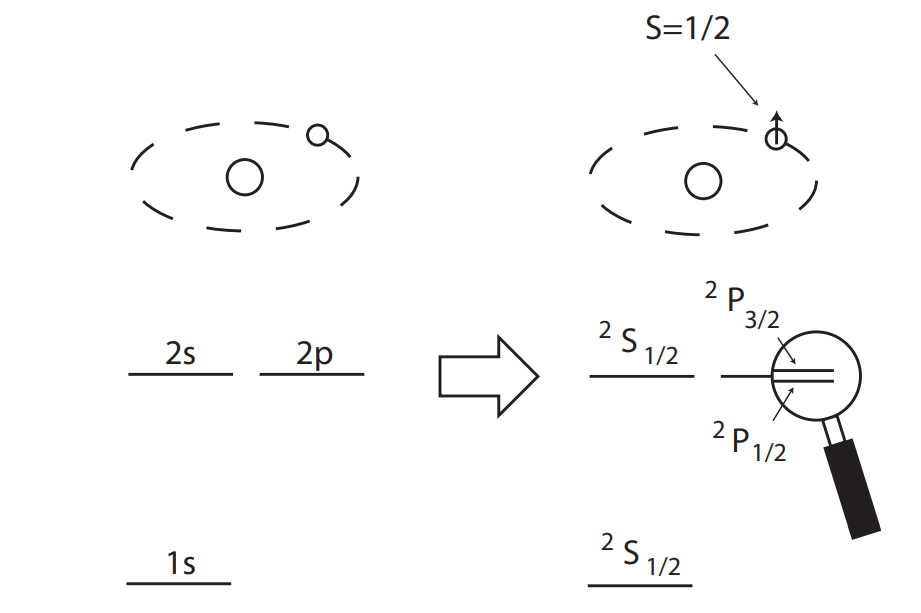
\includegraphics[scale=0.4]{figures/feinstruktur.png}
    \caption{In dieser Abbildung ist die Feinstruktur schematisch dargestellt.\cite{pdf_anleitung}}
    \label{fig:fein}
\end{figure}

\subsection{Hyperfeinstruktur}
Bei der Hyperfeinstruktur wird zusätzlich der Kernspin I betrachtet.
Zusammen mit dem Gesamtdrehimpuls berechnet sich der Gesamtimpuls des Rubidiums mit $\vec{F} = \vec{J} + \vec{I}$.\\
Hierbei ist die Kopplung dieselbe, die auch die Spin-Bahn hat, also berechnet sich die Quantenzahl mit $|I-J|$ bis $|I+J|$.
Es ergeben sich für die zwei Isotope verschiedene Gesamtimpulsquantenzahlen, wie in \autoref{tab:quanten} gelistet ist.
In \autoref{fig:hyper} wird die Hyperfeinaufspaltung von $^{87}\text{Rb}$ dargestellt.\\
Der Grundzustand $^2S_{\sfrac{1}{2}}$ ist in der Abbildung nicht dargestellt, wird jedoch aufgrund des gleichen Gesamtbahndrehimpulses $\text{J}=\sfrac{1}{2}$, auch gleich aufgespalten wie $^2P_{\sfrac{1}{2}}$.

\begin{figure}[H]
    \centering
    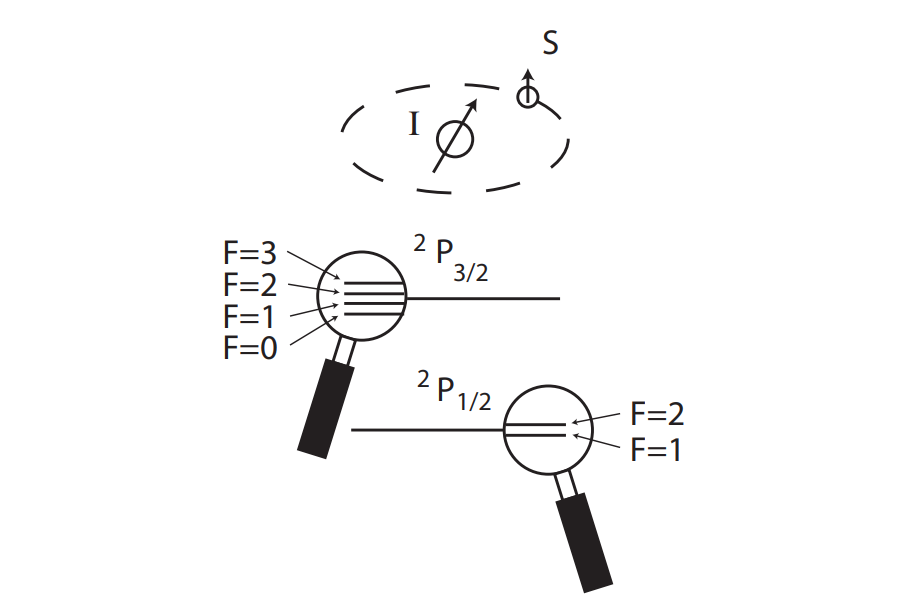
\includegraphics[scale=0.4]{figures/hyperfeinstruktur.png}
    \caption{In dieser Abbildung ist die Hyperfeinstruktur von $^{87}\text{Rb}$ schematisch dargestellt.\cite{pdf_anleitung}}
    \label{fig:hyper}
\end{figure}

\subsection{Zeeman-Aufspaltung}
Die Zeeman-Aufspaltung ist nach dem niederländischen Physiker Pieter Zeeman benannt, der für dessen Entdeckung 1902 den Nobelpreis erhielt.
Der Zeeman Effekt tritt auf, wenn ein äußeres Magnetfeld die Energieniveaus einzelner Zustände von Atomen verschiebt, und dadurch Aufspaltungen in den Spektrallinien bildet.\\
Das äußere magnetfeld wechselwirkt mit der magnetischen Atomhülle, die sich aus der Kopplung von Spin der Elektronen und dem Bahndrehimpuls (L-S-Kopplung) zusammensetzt.
Einen wesentlich kleineren Beitrag leistet der Kernspin I.\\
Die Wechselwirkungsenergie ist gegeben durch:

\begin{equation}
    \Delta E_{\text{Z},F} = g_F \mu_B M B
    \label{eq:zeeman}
\end{equation}
mit dem Bohr'schen Magneton $\mu_B$ und dem Landé-Faktor
\begin{equation}
    g_F = g_J \cdot \frac{F(F+1) + J(F+1) - I(I+1)}{2F(F+1)}
    \quad \text{,} \quad
    g_J = \frac{3J(J+1) + S(S+1) - L(L+1)}{2J(J+1)}
\end{equation}

Die Quantenzahl $M$ beschreibt den aufgespaltenen Zustand, dessen Differenz zum Energieniveau der Hyperfeinaufspaltung das $\Delta E_{\text{Z},F}$ angibt.\\
In \autoref{fig:zeeman} ist die Aufspaltung graphisch dargestellt.

\begin{figure}[H]
    \centering
    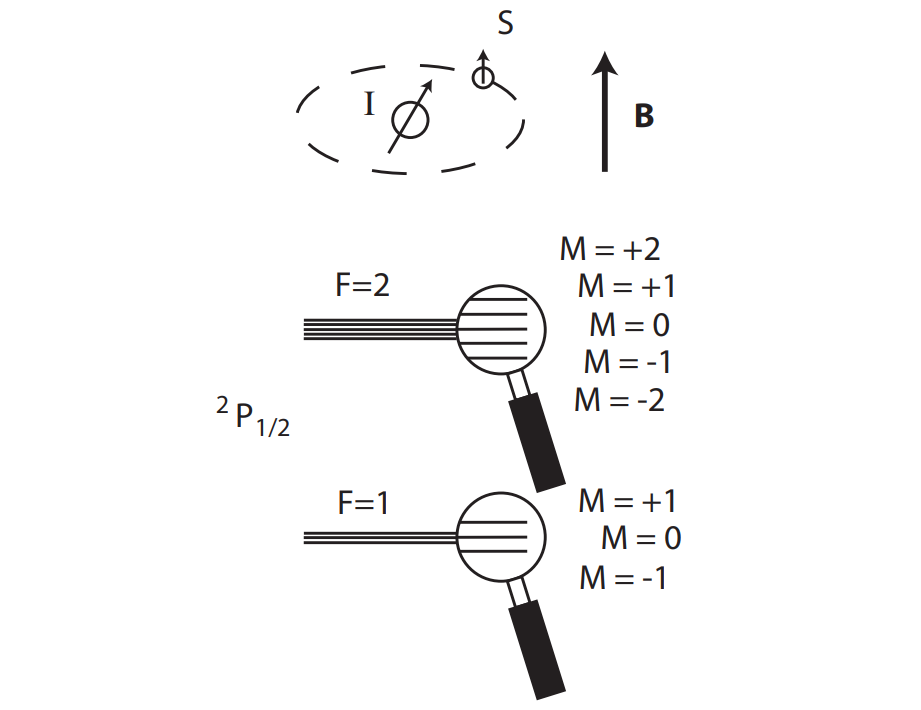
\includegraphics[scale=0.4]{figures/zeeman.png}
    \caption{In dieser Abbildung ist die Zeeman-Aufspaltung von $^{87}\text{Rb}$ graphisch dargestellt.\cite{pdf_anleitung}}
    \label{fig:zeeman}
\end{figure}